\documentclass[12pt,a4paper]{article}

% Required Packages
\usepackage[utf8]{inputenc}
\usepackage{geometry}
\geometry{a4paper, margin=1in}
\usepackage{graphicx}
\usepackage{booktabs}
\usepackage{array}
\usepackage{hyperref}
\usepackage{float}
\usepackage{tikz}
\usetikzlibrary{shapes.geometric, arrows.meta, positioning, calc}
\usepackage{caption}
\usepackage{subcaption}

% TikZ Styles for Block Diagram
\tikzstyle{sensor} = [rectangle, rounded corners, minimum width=2.5cm, minimum height=1cm, text centered, text width=2.5cm, draw=black, fill=blue!10]
\tikzstyle{mcu} = [rectangle, minimum width=3cm, minimum height=4cm, text centered, text width=3cm, draw=black, fill=orange!10]
\tikzstyle{output} = [rectangle, rounded corners, minimum width=2.5cm, minimum height=1cm, text centered, text width=2.5cm, draw=black, fill=green!10]
\tikzstyle{arrow} = [thick,->,>=stealth]

\begin{document}

\begin{titlepage}
    \centering
    
    % Centered Logo
    
\includegraphics[width=3.5cm]{kyu_crest.png}
    \vspace{0.8cm}
    
    {\Large \textbf{FACULTY OF ENGINEERING}}\\[0.2cm]
    {\large DEPARTMENT OF ELECTRICAL AND ELECTRONICS ENGINEERING}\\[0.2cm]
    {\large BACHELORS OF ENGINEERING IN TELECOMMUNICATIONS ENGINEERING}\\[0.5cm]
    
    {\large TETE/TEEE 3102: MICROCONTROLLERS}\\[1cm]
    
    \hrule
    \vspace{0.5cm}
    {\huge \textbf{LAB REPORT}}\\[0.3cm]
    {\LARGE \textbf{SMART ROOM MONITORING SYSTEM}}\\[0.2cm]
    {\Large \textbf{Level 2 Upgrade: Detect, Evidence, Alert \& Power Monitor}}
    \vspace{0.5cm}
    \hrule
    \vspace{1.5cm}
    
    {\Large \textbf{Prepared By:}}
    \vspace{0.5cm}
    
    \begin{center}
        \renewcommand{\arraystretch}{1.2}
        \begin{tabular}{|c|l|c|}
            \hline
            \textbf{No.} & \textbf{Name} & \textbf{Student ID} \\
            \hline
            1 & Mukama Robert & 26/U/ETE/21285/PE \\
            2 & Nabudere Zerubabel & 25/U/ETE/05465/PE \\
            3 & Nanfuka Shakirah & 25/U/ETE/05468/PE \\
            4 & Kidega Wilkie Cephas & 25/U/ETE/05460/PE \\
            \hline
        \end{tabular}
    \end{center}
    
    \vfill
    
    \begin{flushleft}
        \textbf{Course:} TETE/TEEE 3102 \\
        \textbf{Lecturer:} Dr. Dickson Mugerwa \\
        \textbf{Group:} Group 4
    \end{flushleft}
    
    \vspace{-1.5cm}
    \begin{flushright}
        \textbf{Deadline:} 25\textsuperscript{th} August 2026 \\
        \textbf{Date Submitted:} August 31, 2026
    \end{flushright}
    
    \vspace{1cm}
    {\large \textbf{August 2026}}
\end{titlepage}

\newpage
\tableofcontents
\newpage

\section{Introduction: Upgrade from Level 1}
The initial implementation (Level 1) of the Smart Room Monitoring System focused on basic monitoring, local alerts via a buzzer, and data logging to ThingSpeak. 

\textbf{Level 2} significantly upgrades the system capabilities to encompass:
\begin{itemize}
    \item \textbf{Detection:} Advanced intrusion and safety hazard detection.
    \item \textbf{Evidence Capture:} Image capturing capabilities upon motion detection.
    \item \textbf{Alert Anywhere:} Reliable SMS/Call alerts even when Wi-Fi is down.
    \item \textbf{Power Monitoring:} Comprehensive tracking of power consumption and grid status.
\end{itemize}

\section{New Hardware Additions}
To achieve the Level 2 functionalities, the following hardware components have been integrated into the system, bringing the total number of sensors to 7 (DHT22, Ultrasonic, PIR, Camera, Voltage, Current, MQ-2, Reed Switch).

\begin{enumerate}
    \item \textbf{ESP32-CAM (Replacing Arduino Uno/ESP8266):} Utilized for image capture when motion is detected. It has built-in Wi-Fi, efficiently acting as the primary web-connected controller.
    \item \textbf{SIM800L GSM Module:} Critical for the Ugandan context. It sends SMS or initiates phone calls when Wi-Fi is unavailable or for critical security/safety alerts.
    \item \textbf{Voltage Sensor (ZMPT101B) \& Current Sensor (ACS712 20A):} Added to monitor the UEDCL mains. These detect blackouts, over-voltage scenarios, and calculate power consumption in kWh.
    \item \textbf{MQ-2 Gas Sensor:} Deployed in the kitchen area for LPG and smoke leak detection.
    \item \textbf{Magnetic Reed Switch:} Placed on the main door/window for reliable intrusion detection (acting as a robust complement to the PIR sensor).
\end{enumerate}

\section{Hardware Component Visuals}
The physical hardware modules integrated into the Level 2 monitoring system are illustrated below:

\begin{figure}[H]
    \centering
    \begin{subfigure}{0.31\textwidth}
        \centering
        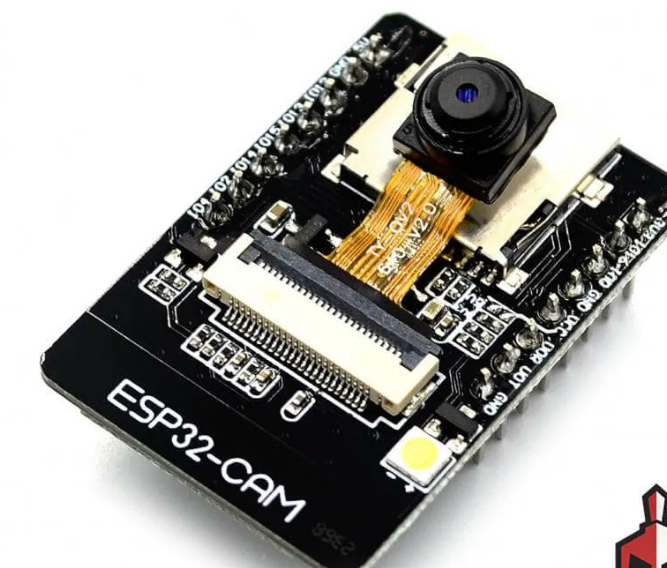
\includegraphics[width=\linewidth,height=3.2cm,keepaspectratio]{espcam.PNG}
        \caption{ESP32-CAM Module}
    \end{subfigure}
    \hfill
    \begin{subfigure}{0.31\textwidth}
        \centering
        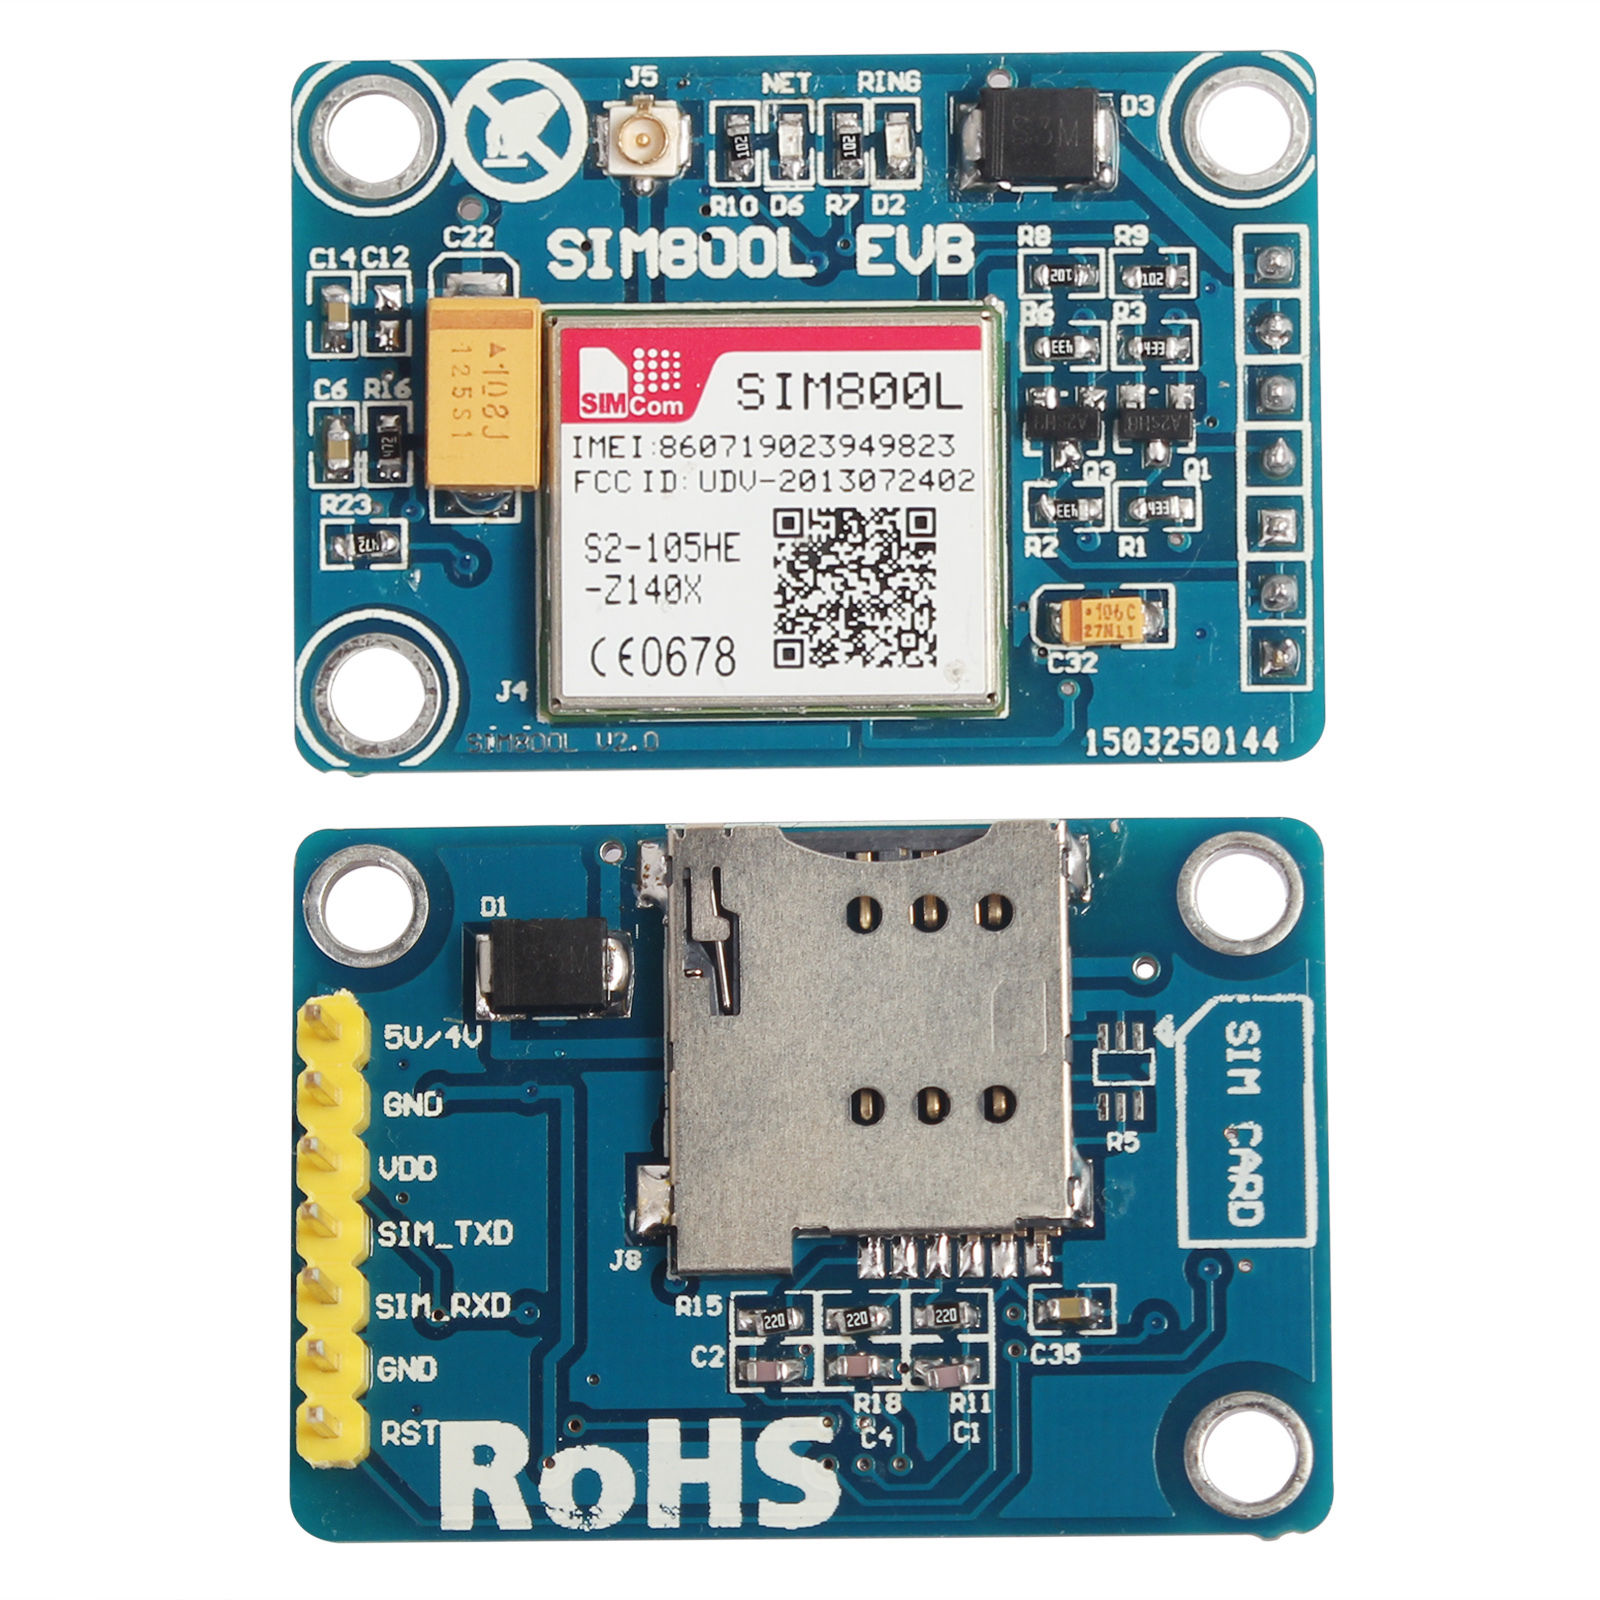
\includegraphics[width=\linewidth,height=3.2cm,keepaspectratio]{GSM-MODULE-SIM800-5V.jpg}
        \caption{SIM800L GSM Module}
    \end{subfigure}
    \hfill
    \begin{subfigure}{0.31\textwidth}
        \centering
        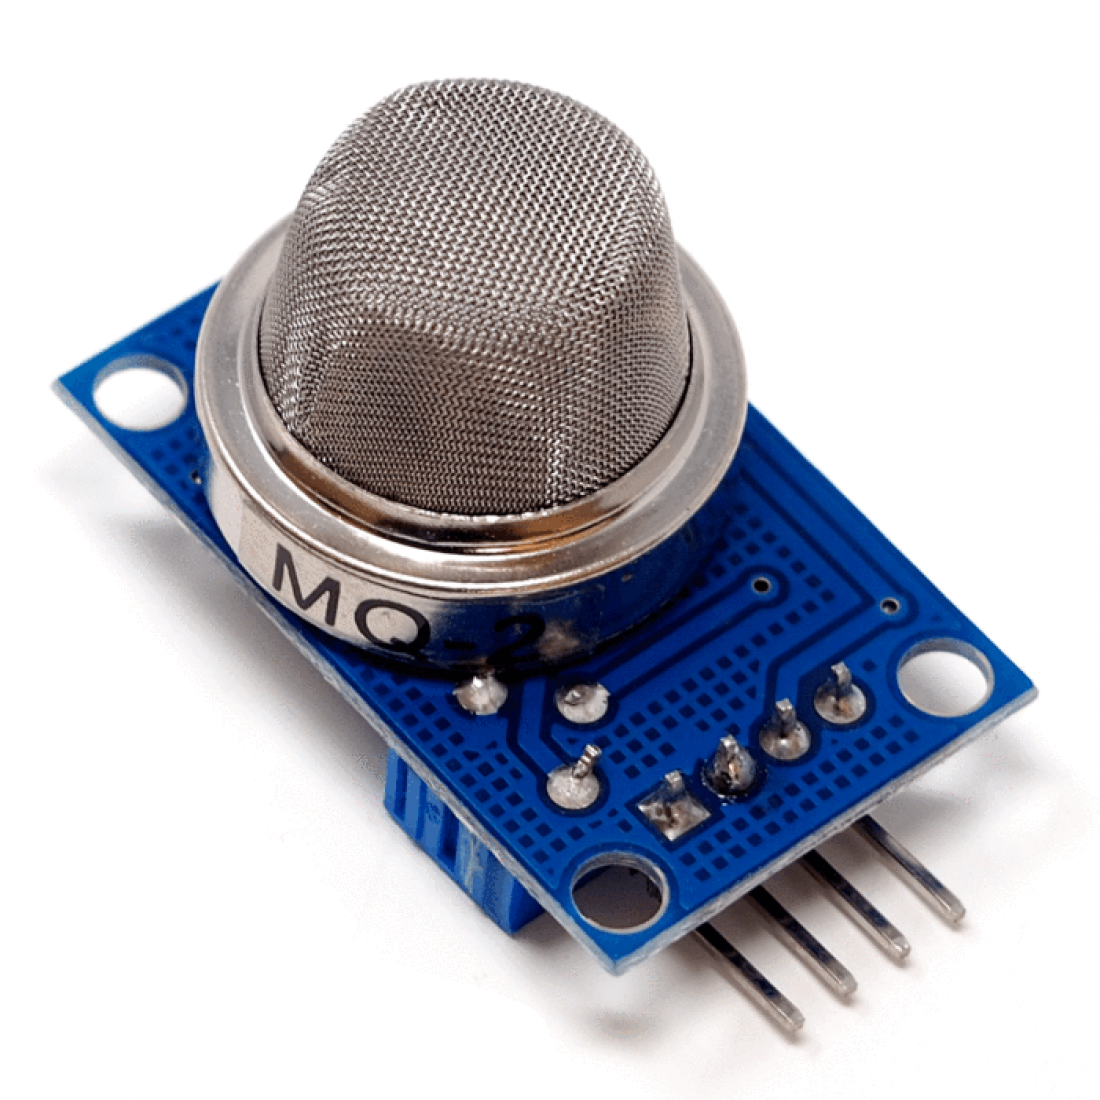
\includegraphics[width=\linewidth,height=3.2cm,keepaspectratio]{mq.png}
        \caption{MQ-2 Gas Sensor}
    \end{subfigure}
    
    \vspace{0.6cm}
    \begin{subfigure}{0.45\textwidth}
        \centering
        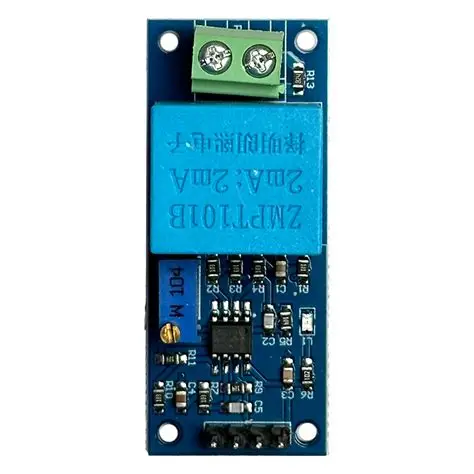
\includegraphics[width=\linewidth,height=3.4cm,keepaspectratio]{ac_volt.png}
        \caption{ZMPT101B AC Voltage Sensor}
    \end{subfigure}
    \hfill
    \begin{subfigure}{0.45\textwidth}
        \centering
        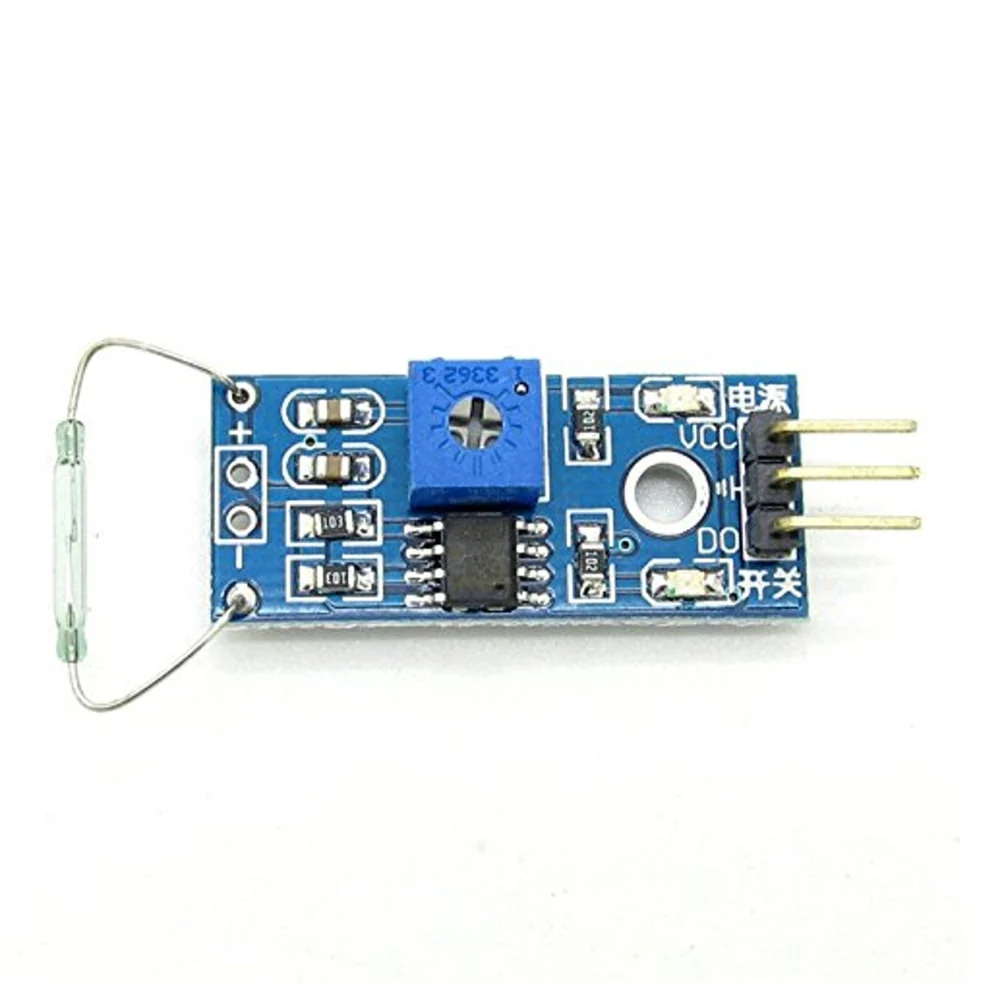
\includegraphics[width=\linewidth,height=3.4cm,keepaspectratio]{reed_switch.png}
        \caption{Magnetic Reed Switch Module}
    \end{subfigure}
    
    \caption{New Hardware Components for Level 2 Upgrade}
    \label{fig:components}
\end{figure}

\section{System Requirements \& Architecture}
The system architecture is divided into four distinct functional layers to ensure robust monitoring and alerting.

\subsection{A. Security Layer}
\begin{itemize}
    \item If the \textbf{Reed Switch} is OPEN or \textbf{PIR = 1} after 10:00 PM, the ESP32-CAM captures an image.
    \item The image is saved to the SD Card and uploaded to a Telegram Bot.
    \item Simultaneously, the GSM module sends an SMS: \textit{“INTRUSION at Door 1 - Time: [HH:MM]”}.
\end{itemize}

\subsection{B. Power Monitoring Layer}
\begin{itemize}
    \item The system continuously reads voltage and current.
    \item If $Voltage < 180V$, $Voltage > 260V$, or $Voltage = 0$ (blackout): Sends an SMS and a ThingSpeak alert.
    \item Calculations: $Power (W) = V \times I$. Cumulative Energy (kWh) is calculated and posted to ThingSpeak Fields 5, 6, and 7.
\end{itemize}

\subsection{C. Safety Layer}
\begin{itemize}
    \item If \textbf{MQ-2} readings exceed the safety threshold (gas leak detected), the Buzzer turns ON continuously.
    \item The GSM module initiates a phone call.
    \item A relay is activated to trigger an exhaust fan or open a window.
\end{itemize}

\subsection{D. Data Layer}
\begin{itemize}
    \item The \textbf{ThingSpeak Channel} is upgraded to utilize 8 fields: Temperature, Humidity, Distance, Motion, Voltage, Current, Power, and Gas Level.
    \item \textbf{Blynk} or \textbf{Telegram} is implemented for real-time control and system status queries.
\end{itemize}

\section{System Block Diagram}
Below is the block diagram representing the data flow and interconnections between the 7 sensors, the core processing unit, and the output interfaces.

\begin{figure}[H]
    \centering
    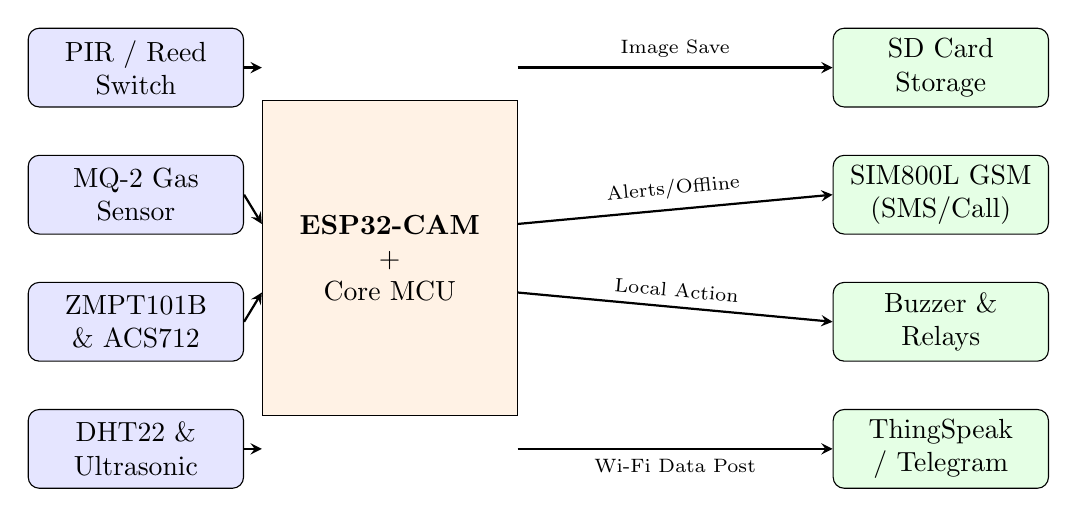
\begin{tikzpicture}[
        node distance=0.8cm and 1.8cm,
        every text node part/.style={align=center}
    ]
        
        % Sensors (Left Column)
        \node (pir) [sensor] {PIR / Reed Switch};
        \node (mq2) [sensor, below=0.6cm of pir] {MQ-2 Gas Sensor};
        \node (power) [sensor, below=0.6cm of mq2] {ZMPT101B \& ACS712};
        \node (dht) [sensor, below=0.6cm of power] {DHT22 \& Ultrasonic};
        
        % MCU (Center Column)
        \path (pir) -- (dht) coordinate[midway] (sensormid);
        \node (mcu) [mcu, right=1.6cm of sensormid] {\textbf{ESP32-CAM} \\ + \\ Core MCU};
        
        % Outputs (Right Column)
        \node (sd) [output, right=2.0cm of pir] at ([xshift=2.0cm]mcu.east |- pir) {SD Card Storage};
        \node (gsm) [output, below=0.6cm of sd] {SIM800L GSM (SMS/Call)};
        \node (relay) [output, below=0.6cm of gsm] {Buzzer \& Relays};
        \node (cloud) [output, below=0.6cm of relay] {ThingSpeak / Telegram};
        
        % Arrows: Sensors -> MCU
        \draw [arrow] (pir.east) -- (mcu.west |- pir);
        \draw [arrow] (mq2.east) -- (mcu.165);
        \draw [arrow] (power.east) -- (mcu.195);
        \draw [arrow] (dht.east) -- (mcu.west |- dht);
        
        % Arrows: MCU -> Outputs
        \draw [arrow] (mcu.east |- sd) -- (sd.west) node[midway, above, font=\scriptsize] {Image Save};
        \draw [arrow] (mcu.15) -- (gsm.west) node[midway, above, sloped, font=\scriptsize] {Alerts/Offline};
        \draw [arrow] (mcu.345) -- (relay.west) node[midway, above, sloped, font=\scriptsize] {Local Action};
        \draw [arrow] (mcu.east |- cloud) -- (cloud.west) node[midway, below, font=\scriptsize] {Wi-Fi Data Post};
        
    \end{tikzpicture}
    \caption{Level 2 Architecture Block Diagram}
    \label{fig:block_diagram}
\end{figure}

\section{Deliverables}
The finalized project submission includes the following deliverables:
\begin{enumerate}
    \item \textbf{Block Diagram \& Fritzing Circuit:} Detailed schematic and architectural overview.
    \item \textbf{Working Prototype:} Physical assembly of all 7 sensors, GSM, and ESP32-CAM.
    \item \textbf{Live Dashboard Link:} ThingSpeak and Telegram bot access containing at least 48 hours of live logged data.
    \item \textbf{Costing Analysis:} A Bill of Materials (BOM) cost estimation for a hypothetical deployment of 100 units.
\end{enumerate}

\end{document}
